\subsection{Timing Capacitor and Resistor}\label{Timing Capacitor and Resistor}
\textcolor{gray}{De oscillator frequentie wordt gegeven door de timig weerstand en timing condensator en is gerelateerd door: }
\textcolor{gray}{
\begin{equation}
F_{osc} = \frac{1.72}{R_t\cdot C_T }
\label{Eq_Fosc}
\end{equation}
}

\textcolor{gray}{Ook kan de timing condensator en weerstand gelezen worden van \autoref{fig:Datasheet_timing_res_cap_switch_freq}}

\begin{figure}[!h]
    \centering
    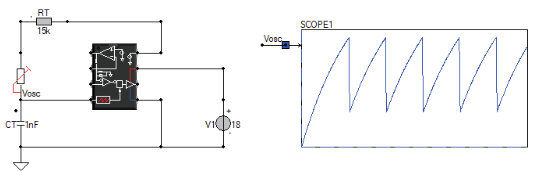
\includegraphics[width=0.5\linewidth]{img//hfd3/Variable oscillator frequency.png}
    \caption{Variable oscillator frequency}
    \label{fig:Variable oscillator frequency}
\end{figure}

\begin{figure}[!h]
    \centering
    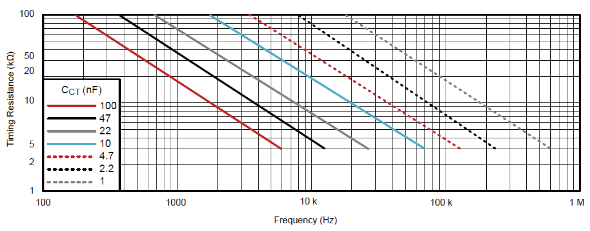
\includegraphics[width=0.5\linewidth]{img//hfd3/Datasheet showing resistor RT and capacitor CT for defining the switching frequency.png}
    \caption{Datasheet showing resistor RT and capacitor CT for defining the
switching frequency}
    \label{fig:Datasheet_timing_res_cap_switch_freq}
\end{figure}